\chapter{Complexidade Computacional}

% Funções de complexidade, que satisfazem aos axiomas de Blum
\newcommand{\PhiDT}{{\mathcal{T}}} % Tempo determinístico
\newcommand{\PhiDS}{{\mathcal{S}}} % Espaço determinístico
\newcommand{\PhiNT}{{\mathcal{N\!T}}} % Tempo não-determinístico
\newcommand{\PhiNS}{{\mathcal{N\!S}}} % Espaço não-determinístico

\emph{Complexidade} é a quantidade de recursos
que uma máquina de Turing gasta
para computar determinada função
ou para decidir pertinência a uma linguagem
\cite[p.~285]{HopcroftUllman1979}.
Os recursos mais importantes para a teoria de complexidade computacional
são o espaço e o tempo,
em máquinas de Turing determinísticas e não"=determinísticas.

Os axiomas de Blum definem a noção de complexidade computacional
não apenas para máquinas de Turing,
mas sim para qualquer modelo de computação que satisfaça algumas restrições.

A seção~\ref{sec:enumeration_of_recursive_functions}
contém a maquinaria matemática necessária para expressar estas restrições.
Os axiomas de Blum aparecem na seção~\ref{sec:blum_axioms}.
Por fim, a seção~\ref{sec:default_measures}
define as medidas de complexidade padrão.

\section{Teoria de Complexidade Axiomática: Axiomas de Blum}
\label{sec:blum_axioms}

\begin{definition}
    Seja $\phi$ uma enumeração de Gödel aceitável.
    Uma \emph{medida de complexidade} é uma função
    $\Phi: \{0, 1\}^* \times \{0, 1\}^* \to \mathbb N$,
    que satisfaz aos seguintes axiomas:\footnotemark
    \begin{enumerate} [label=\textbf{Axioma \arabic*}, ref=\arabic*, align=left]
        \item
            \label{ax:blum_def}
            $\Phi(x, y)$ está definido
            se, e somente se,
            $\phi_x(y)$ está definido.
        \item
            \label{ax:blum_rec}
            A função $R(x, y, m)$,
            definida como $1$ se $\Phi(x, y) = m$,
            e $0$ caso contrário,
            é recursiva total.
    \end{enumerate}

    \footnotetext{
        A definição original de \citeonline[p.~3]{Blum1967}
        é dada no contexto do cálculo de funções de inteiros.
        Em particular,
        as enumerações de Gödel aceitáveis são indexadas por números,
        não por cadeias de $\{0, 1\}^*$.
        Esta adaptação é baseada na definição de \citeonline[p.~156]{Papadimitriou1994}.
    }
\end{definition}

O axioma~\ref{ax:blum_rec}
nos dá um semialgoritmo para calcular $\Phi(x, y)$.
Entretanto, pelo axioma~\ref{ax:blum_def},
não podemos ir muito além disso,
pois $\phi_x(y)$ não está definido para todo $x$ e $y$.
(De fato, decidir se $\Phi(x, y)$ existe
é exatamente o problema da parada para o modelo de computação de $\phi$.)

Nos exemplos que se seguem,
quando estivermos usando a enumeração de Gödel $f_x$,
utilizaremos a notação $\Phi(\langle M \rangle, x)$
para nos referir a $\Phi(w, x)$,
em que $w$ é a codificação (em binário) da máquina $M$.
Não há problemas de ambiguidade,
pois a codificação $w = \langle M \rangle$ como definida
identifica a função $f_w$ unicamente.

\begin{example}
    \label{ex:time_complexity}
    \simbolo{$\PhiDT$}{Complexidade de Tempo}
    A \emph{complexidade de tempo},
    que denotaremos por $\PhiDT$,
    é a função que diz quantos movimentos
    uma máquina de Turing faz até retornar uma resposta.
    Isto é,
    \begin{equation*}
        \PhiDT( \langle M \rangle, x ) = \begin{cases}
            k, & \text{
                \parbox{0.6\textwidth}{
                    se $M$ executa exatamente $k$ passos em $x$ antes de parar.
                }
            } \\
            \text{indefinido}, & \text{
                \parbox{0.6\textwidth}{
                    caso $M$ nunca pare de computar $x$.
                }
            }
        \end{cases}
    \end{equation*}
    Para determinar se $\PhiDT( \langle M \rangle, x) = k$,
    execute a máquina $M$ por $k$ passos
    e veja se é a primeira vez que
    $M$ atinge um estado aceitador.
    E, como $\PhiDT( \langle M \rangle, x)$ só está definido se $M$ para ao computar $x$,
    $\PhiDT$ satisfaz aos dois axiomas de Blum.
\end{example}

\begin{example}
    \label{ex:space_complexity}
    \simbolo{$\PhiDS$}{Complexidade de Espaço}
    Para a \emph{complexidade de espaço},
    que denotaremos por $\PhiDS$,
    assumiremos que $M$ possui uma fita somente"=leitura
    específica para a entrada.
    \begin{equation*}
        \PhiDS( \langle M \rangle, x) = \begin{cases}
            k, & \text{
                \parbox{0.6\textwidth}{
                    se~$M$ para ao computar~$x$,
                    tendo lido exatamente~$k$ células
                    de uma de suas fitas de trabalho
                    e no máximo $k$~células nas demais fitas.
                }
            } \\
            \text{indefinido}, & \text{
                \parbox{0.6\textwidth}{
                    se $M$ nunca parar ao computar $x$.
                }
            }
        \end{cases}
    \end{equation*}
    Precisamos desta definição intrincada
    pois~$M$ pode não ler $k$~células de todas as suas fitas,
    apenas de algumas.

    Claramente o axioma~\ref{ax:blum_def} é satisfeito.
    Para o axioma~\ref{ax:blum_rec},
    o algoritmo é um pouco mais complicado.

    Comece executando $M$ em $x$.
    Caso $M$ extrapole $k$ células lidas
    em alguma de suas fitas,
    podemos rejeitar a entrada
    (isto é, $\Phi(\rangle M \langle, x) = k$ é falso).
    Caso contrário,
    existirá um número finito de configurações da máquina.

    Existem~$|\Gamma|^k$ possíveis fitas com $k$ termos
    e $k+1$ possíveis posições da cabeça de leitura;
    teremos, portanto,
    $(k+1)|\Gamma|^k$~diferentes configurações para cada fita.
    Para $l$ diferentes fitas e $|Q|$~possíveis estados da máquina,
    existem, no máximo,
    \begin{equation}
        |Q| \left((k+1)|\Gamma|^k\right)^l
        \label{eq:configurations_count}
    \end{equation}
    possíveis configurações.
    Portanto, se a máquina executar
    mais movimentos do que este número,
    significa que ela entrou em loop.
    Podemos rejeitar a entrada.%
    \footnote{
        Este cuidado adicional é imprescindível
        para garantir que o predicado
        ``$\Phi(\langle M \rangle, x) = k$''
        seja decidível,
        não apenas semidecidível.

        Note que precisamos rejeitar a entrada
        caso a máquina entre em loop
        porque $\Phi( \langle M \rangle, x)$ só está definido
        quando $M(x)$ está
        --- não é o caso se $M$ entra em loop
        ao computar $x$.
    }

    E, por último,
    caso $M$ pare,
    precisamos nos assegurar que,
    de fato,
    em alguma das fitas $k$ células foram lidas.
\end{example}

\begin{example}
    \label{ex:nondeterministic_complexity}
    \simbolo{$\PhiNT$}{Complexidade de Tempo não"=determinística}
    \simbolo{$\PhiNS$}{Complexidade de Espaço não"=determinística}
    Podemos adaptar $\PhiDT$ e $\PhiDS$
    para máquinas de Turing não"=determinísticas.%
    \footnote{
        Tecnicamente,
        as denominações usuais,
        ``complexidade de tempo/espaço não"=determinística''
        ou ``tempo/espaço não"=determinístico''
        estão erradas;
        não é o tempo ou espaço ou a complexidade que são não"=determinísticos,
        mas sim o modelo de máquina ao qual nos referimos.

        Entretanto, toleraremos este abuso de nomenclatura neste texto.
    }

    A complexidade de tempo não"=determinística,
    que denotaremos por $\PhiNT(\langle M \rangle, x)$,
    definiremos como sendo a maior quantidade de movimentos
    tomadas por $M$ ao computar $x$
    dentre todas as escolhas de transições possíveis.

    Analogamente,
    definiremos a complexidade de espaço não"=determinística,
    que denotaremos por $\PhiNS(\langle M \rangle, x)$,
    como sendo a maior quantidade de células lidas
    em qualquer dos ramos da computação de $M$ em $x$.
    Aqui, precisamos tomar o mesmo cuidado que tomamos
    com $\PhiDS$ para demonstrar o axioma~\ref{ax:blum_rec}.
\end{example}

Nos exemplos \ref{ex:time_complexity} e~\ref{ex:space_complexity},
a enumeração utilizada é a $f_x$
definida na seção~\ref{sec:definition_enumeration_of_recursive_functions}.
No exemplo~\ref{ex:nondeterministic_complexity},
ficou faltando definir a enumeração de Gödel associada;
isto é, jogamos o problema de
explicar como uma máquina não"=determinística computa uma função
para ``debaixo do tapete''.
Voltaremos a este problema no capítulo~\ref{ch:nondeterministic_functions}.
Por ora,
será suficiente nos restringirmos às funções booleanas,
usando a mesma definição usada para decisores.

\begin{example}
    Escolher $\Phi(w, x) = 0$ para todo $M$ e $x$
    satisfaz ao axioma~\ref{ax:blum_rec},
    mas não ao axioma~\ref{ax:blum_def},
    pois $\Phi(w, x)$ está definida mesmo quando $f_w(x)$ não está.
    Já definir $\Phi(w, x) = |f_w(x)|$
    satisfaz ao axioma~\ref{ax:blum_def},
    mas não ao axioma~\ref{ax:blum_rec},
    pois poderíamos resolver o problema da parada:
    dada uma máquina $M$, podemos modificá"=la
    para apagar sua fita logo antes de parar.
    Então, para esta $M'$,
    $\Phi(\langle M' \rangle, x) = 0$ se, e somente se,
    a $M$ original para ao computar $x$.
    Estes dois exemplos mostram que os axiomas são independentes
    \cite[p.~3]{Blum1967}.
\end{example}

Podemos ver que as medidas $\PhiDT$ e $\PhiDS$ estão relacionadas.
Para ler uma posição da fita,
é necessário gastar ao menos uma unidade de tempo.
Ou seja,
\begin{equation*}
    \PhiDS(\langle M \rangle, x) \leq \PhiDT(M, x).
\end{equation*}
E, de acordo com o raciocínio do exemplo~\ref{ex:space_complexity},
para todo $M$ existe algum $c$ que
\begin{equation*}
    \PhiDT(\langle M \rangle, x) \leq c^{\PhiDS(M, x)}.
\end{equation*}
De fato, podemos relacionar quaisquer duas medidas de complexidade.

\begin{theorem}
    \label{thm:measure_related}
    Dada uma enumeração de Gödel aceitável $\phi$
    e duas medidas de complexidade $\Phi$ e $\hat \Phi$ para $\phi$,
    existe uma função recursiva $r$ tal que
    \begin{equation*}
        \Phi(w, x) \leq r( x, \hat \Phi(w, x))
    \end{equation*}
    para todo $w$ e quase todo $x$.%
    \footnote{
        Um predicado é ``verdadeiro para quase todo $n$''
        quando ele é falso para apenas uma quantidade finita de números $n$.
        Equivalentemente,
        é quando existe algum $n_0$ tal que
        o predicado é válido para todo $n > n_0$.
    }
\end{theorem}

\begin{proof}
    Defina
    \begin{equation*}
        r( x, k ) = \max \{ \Phi(w, x) \mid |w| \leq |x| \land \hat \Phi(w, x) = k \}
    \end{equation*}
    Fixado $x$, existe um número finito de máquinas de Turing
    cuja descrição é menor que $|x|$.
    O conjunto na definição acima é um subconjunto desta lista
    (pois, além da exigência $|w| \leq |x|$,
    exigimos que $\hat \Phi(w, x) = k$.)

    O predicado $\hat \Phi(w, x) = k$ é recursivo.
    Quando este predicado é verdadeiro,
    $\phi_w(x)$ está definido, pelo axioma~\ref{ax:blum_def},
    portanto $\Phi(w, x)$ também está definido e pode ser calculado.
    Concluímos que $r$ é recursiva.

    Agora, para todos os $x$ que são mais longos que $w$,
    $\Phi(w, x)$ será um dos elementos do conjunto acima
    para $r(x, \hat \Phi(w, x))$,
    portanto é menor ou igual a $\Phi(w, x)$.
\end{proof}

\citeonline[p.~4]{Blum1967} demonstra uma versão ligeiramente mais forte
deste teorema.
Ele prova que $r$ pode ser tal que,
simultaneamente,
\begin{equation*}
    \Phi(w, x) \leq r( x, \hat \Phi(w, x))
\end{equation*}
e
\begin{equation*}
    \hat \Phi(w, x) \leq r( x, \Phi(w, x))
\end{equation*}
Podemos construir uma função dessas
pegando o máximo de duas funções obtidas
usando o teorema~\ref{thm:measure_related}.

O teorema,
assim como provamos,
não pode ser fortalecido
para que $r$ seja uma função de apenas uma variável.
Considere $A$ uma máquina de Turing
que opere como um autômato finito.
$\PhiDT(\langle A \rangle, x) = |x|$ para toda palavra $x$,
enquanto que $\PhiDS(\langle A \rangle, x) = 1$ para toda palavra $x$.%
\footnote{
    A complexidade de espaço não é $0$
    pois $A$ é obrigada a ler
    ao menos a célula inicial da sua fita de trabalho,
    embora a máquina não use aquela célula.
}
Se $r$ pudesse depender apenas da segunda variável,
isto é, $r(x, k) = r'(m)$ para alguma função $r'$,
teríamos
\begin{align*}
    |x| &= \PhiDT(\langle A \rangle, x) \\
        &\leq r(x, \PhiDS(\langle A \rangle, x)) \\
        &= r(x, 1) \\
        &= r'(1)
\end{align*}
que é falso para todo $x$ suficientemente comprido.

Caso $r$ pudesse depender apenas da primeira variável,
isto é, $r(x, k) = r''(x)$ para alguma função $r''$,
teríamos, para todas as máquinas de Turing,
\begin{equation*}
    \PhiDT(\langle M \rangle, x) \leq r''(x).
\end{equation*}
Mas, como $r''$ é recursiva
(pois $r$ o é),
podemos construir uma máquina que calcula $r''(x)$,
desperdiça $r''(x)$ movimentos,
e aceita a entrada.
Para esta $M'$,
\begin{equation*}
    \PhiDT(\rangle M' \langle, x) > r''(x),
\end{equation*}
contradizendo a equação anterior.

No parágrafo anterior,
construímos uma máquina de Turing
que deliberadamente desperdiça tempo
ao computar determinada função.
\citeonline[p.~4]{Blum1967} demonstrou que
é sempre possível desperdiçar recursos computacionais,
quaisquer que sejam estes recursos.
Precisamos de um lema,
vindo direto da teoria das funções recursivas.

\begin{lemma}[Teorema da Recursão]
    Para qualquer enumeração de Gödel aceitável $\phi$
    e qualquer função recursiva total $\sigma$,
    existe um valor $w$ tal que
    \begin{equation*}
        \phi_w(x) = \phi_{\sigma(w)}(x)
    \end{equation*}
    para todo $x$.
    (Tal valor é chamado de \emph{ponto fixo} para $\sigma$.)
    \label{thm:recursion}
\end{lemma}

\begin{proof}
    Ilustraremos o teorema com o caso $\phi_x = f_x$.
    %TODO: Demonstrar por completo.

    Primeiro, construiremos uma máquina $M$ que,
    ao receber $x$ na entrada,
    computará uma máquina equivalente a $\phi_x(x)$.
    Isto é, para todo $y$,
    \begin{equation}
        \phi_{M(x)}(y) = \phi_{f_x(x)}(y),
        \label{eq:diagonal_N}
    \end{equation}
    sempre que $f_x(x)$ existir.
    \footnotetext{
        Duas palavras $u$ e $v$ são equivalentes
        se, para todo $x$, $f_u(x) \simeq f_v(x)$.
    }

    A abordagem direta,
    calcular $\phi_x(x)$,
    não funciona,
    pois $\phi_x(x)$ pode não existir.
    pois a máquina representada por $x$ pode nunca parar ao processar $x$.

    Observe que não precisamos retornar $M_x(x)$,
    e sim, apenas uma máquina equivalente a $M_x(x)$,
    caso $M_x(x)$ exista.
    Na entrada $x$, $N$ retornará uma máquina que,
    ao receber $y$ na entrada,
    compute $M_x(x)$,
    e, somente após $M_x$ retornar,
    rode $M_x(x)$ em $y$
    (usando uma máquina de Turing universal).

    É importante notar que $N$ sempre pára;
    $M_x(x)$ pode não parar ao computar $x$,
    mas isso significa, apenas,
    que $N(x)$ nunca parará ao computar qualquer coisa
    --- o valor $N(x)$ existirá.

    De posse da máquina $N$, podemos prosseguir.
    Escolha $k$ como sendo um índice para $\sigma \circ N$.
    Isto é,
    \begin{equation}
        M_k(x) = \sigma(N(x))
        \label{eq:k_sigma_N}
    \end{equation}
    para todo $x$.
    Afirmamos que $m = N(k)$
    satisfaz às exigências do teorema.

    De fato,
    \begin{align*}
        M_m(x) &= M_{N(k)}(x) \\
               &= M_{M_k(k)}(x) && \text{Pela equação~\ref{eq:diagonal_N}}\\
               &= M_{\sigma(N(k))}(x) && \text{Pela equação~\ref{eq:k_sigma_N}}\\
               &= M_{\sigma(m)}(x) && \text{Pela definição de $m$.}
    \end{align*}
\end{proof}

\begin{proposition}
    Seja $\phi$ uma numeração de Gödel aceitável,
    $\Phi$ uma medida de complexidade para $\phi$,
    e $f$ e $g$ funções recursivas totais.
    (Interpretaremos $g$ como sendo uma função de inteiros.)
    Então existe um índice $w$ para a função $f_w$ tal que
    \begin{equation*}
        \Phi(w, x) > g(\langle|x|\rangle)
    \end{equation*}
    para todo $x$.
    \label{thm:resource_waste}
\end{proposition}

Ou seja,
o dispositivo computacional representado por $w$
desperdiça mais de $g(n)$ unidades do recurso medido por $\Phi$
ao processar uma palavra de tamanho $n$.
Em outras palavras,
código ruim pode ser feito em qualquer linguagem.

\begin{proof}
    Defina a função $h$, de duas variáveis, por
    \begin{equation*}
        h(w, x) = \begin{cases}
            \phi_w(x)1 & \text{se $\Phi(w, x) \leq g(\langle|x|\rangle)$} \\
            f(x) & \text{caso contrário.}
        \end{cases}
    \end{equation*}
    ($\phi_w(x)a$ é o valor de $\phi_w(x)$ concatenado com o símbolo $1$.)

    Observe que $h$ é uma função computável,
    pois $\Phi$, $g$ e $f$ o são,
    e, caso $\Phi(w, x)$ esteja definido,
    $\phi_w(x)$ também estará.

    Seja $S$ a função $S_{mn}$ da enumeração $\phi$,
    e $v$ um índice para $h$.
    Construa a função $\sigma$ que,
    na entrada $w$, calcula $S(v, w)$
    --- isto é, $\sigma(w) = S(v, w)$.
    Portanto,
    \begin{equation*}
        \phi_{\sigma(w)}(x) = \phi_{S(v, w)}(x) = \phi_v(\langle w, x \rangle) = h(w, x).
    \end{equation*}
    Observe que $\sigma$ é recursiva total, pois $S$ o é.

    Pelo teorema da recursão (lema~\ref{thm:recursion}),
    $\sigma$ possui um ponto fixo $w_0$.
    Demonstraremos que $w_0$ satisfaz às exigências do teorema.

    Caso a função $h$, ao computar o valor de $h(w_0, x)$
    para algum $x$,
    tenha escolhido a primeira cláusula,
    a saída final de $\sigma(w_0)$ teria sido
    $\phi_{w_0} (x)$ concatenado com $1$,
    que é diferente de apenas $\phi_{w_0}(x)$.
    Portanto, $w_0$ não seria um ponto fixo de $\sigma$,
    contradizendo o teorema da recursão.

    Portanto, $h$ nunca seleciona a primeira cláusula
    ao computar $h(w_0, x)$, para qualquer $x$.
    Isto significa que $\Phi(w_0, x) > g(\langle |x| \rangle)$ para todo $x$,
    o que garante a exigência de complexidade,
    e que
    \begin{equation*}
        \phi_{\sigma(w_0)}(x) = f(x).
    \end{equation*}
    Mas, como $w_0$ é um ponto fixo de $\sigma$,
    a própria $w_0$ já computava $f$ antes de passar por $\sigma$,
    o que prova a exigência da função.
\end{proof}

\subsection{Classes de Complexidade}

\begin{definition}
    Dada uma medida de complexidade $\Phi$
    e uma função recursiva total
    $f: \mathbb N \rightarrow \mathbb N$,
    a \emph{classe de complexidade $f$} com relação a $\Phi$
    é o conjunto
    \begin{equation*}
        \mathcal C_\Phi(f) = \{ L(M) \mid \Phi(M, x) \leq f(|x|)
            \text{ para quase todos os $x$}
        \}.
    \end{equation*}
\end{definition}
Permitiremos que a complexidade de $M$
possa ser maior que $f$ para um número finito de elementos
para simplificar as demonstrações.

Embora faça sentido definir $\mathcal C_\Phi(f)$
para funções $f$ arbitrárias,
a exigência de $f$ ser recursiva total
torna as classes de complexidade
suscetíveis a argumentos por diagonalização.

Por exemplo,
podemos mostrar que
nenhuma classe de complexidade contém todas as linguagens recursivas.
Precisamos de um lema.

\begin{lemma}
    Existe um mapeamento bijetivo computável
    entre $\mathbb N$ e $\mathbb N \times \mathbb N$.
\end{lemma}

\begin{proof}
    Percorra o caminho descrito pelas setas na figura~\ref{passeio_cantor}.

    \begin{figure}[h]
        \centering
        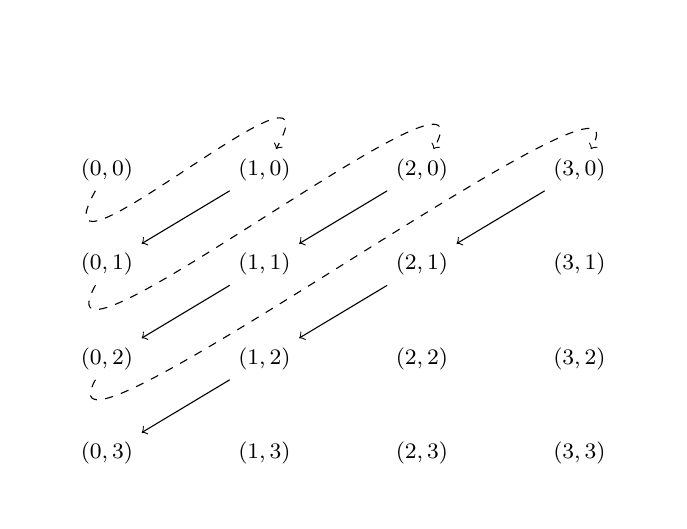
\begin{tikzpicture}
            \foreach \i in {0,...,3}
            \foreach \j in {0,...,3} {
                \node[font=\footnotesize]
                    (a\i\j) at (2*\i, -1.2*\j) {$(\i, \j)$};
            }

            \foreach \a/\b in {a00/a10, a01/a20, a02/a30} {
                \draw[->, dashed] (\a) .. controls
                +(-1,-1.8) and
                +(1, 1.8) .. (\b);
            }

            \foreach \a/\b in {
                a10/a01, a20/a11, a11/a02,
                a30/a21, a21/a12, a12/a03%
            } {
                \draw[->] (\a) -- (\b);
            }
        \end{tikzpicture}
        \caption{Passeio de Cantor.}
        \label{passeio_cantor}
    \end{figure}

    Em essência, primeiro enumeraremos todas os pares $(m, n)$
    para os quais $m + n = 0$,
    depois todos aqueles que $m + n = 1$,
    depois todos os que $m + n = 2$,
    e assim por diante.

    Esta técnica é conhecida como ``passeio de Cantor''
    \cite[p.~6]{CarnielliConiglioBianconi2006}.
\end{proof}

\begin{lemma}
    Existe uma função sobrejetora computável
    $f: \mathbb N \rightarrow \mathbb N$
    tal que,
    para todo $y$,
    existem infinitos $x$ tais que $f(x) = y$.
\end{lemma}
\begin{proof}
    Considere $g$ como a função do lema anterior,
    e defina
    \begin{equation*}
        f(x) = y \quad \text{se} \quad g(x) = (y, z).
    \end{equation*}
\end{proof}

\begin{lemma}
    Existe uma máquina de Turing $N$
    tal que $N(x)$ sempre está definido,
    e representa uma máquina de Turing,
    de forma que toda \emph{representação}
    de uma máquina de Turing
    é $N(x)$ para infinitamente muitos $x$.
    Isto é, $N$ produz todas as representações de máquinas de Turing
    infinitas vezes,
    conforme permitimos que $x$ tome valores arbitrários de $\Sigma^*$.
\end{lemma}

\begin{proof}
    Observe que existe uma bijeção computável
    entre palavras de $\Sigma^*$
    e números naturais.
    $N$ computará,
    dado um $x$,
    o número natural equivalente a ele
    e usar a função do lema anterior
    para gerar outro número.
    Então, $N$ converterá este outro número
    novamente para uma palavra de $\Sigma^*$.

    Todas as palavras de $\Sigma^*$
    são representações de máquinas de Turing;
    portanto, esta palavra produzida é a máquina desejada.

    Como a função do lema anterior
    produz todos números naturais infinitas vezes
    (e $N$ é capaz de suprir todos os números naturais
    como entrada para aquela função),
    todas as representações de máquinas de Turing
    são produzidas por $N$ infinitas vezes.
\end{proof}

\begin{theorem}
    Seja $\mathcal C_\Phi(f)$ uma classe de complexidade
    com relação à $\Phi$.
    Então existe uma linguagem $L$
    que não pertence à esta classe de complexidade.
    \label{funcao_fora_classe}
\end{theorem}

\begin{proof}
    Construiremos uma linguagem $L$
    que discorda de todas as máquinas de Turing que gastam menos de
    $f(n)$ recursos ao computar uma palavra de tamanho $n$.

    Usaremos a máquina $N$ do lema anterior.
    Denotaremos por $M_x$
    a máquina de Turing que $N$ produz
    ao lhe ser dada a palavra $x$.
    Colocaremos $x$ em $L$
    de acordo com o comportamento que $M_x$ tem ao computar $x$.
    Caso esta máquina encerre sua computação
    gastando no máximo $f(|x|)$ recursos,
    executaremos"-na até o final da computação
    e inverteremos o resultado:
    se $M_x$ aceita $x$, então $x \notin L$;
    se $M_x$ rejeita $x$, então $x \in L$.
    Caso $M_x$ exija mais do que $f(|x|)$ recursos,
    coloque $x$ em $L$.
    \footnote{
        Este argumento é,
        de certa forma,
        uma versão limitada
        (por $f$)
        do problema da parada.
    }

    Em outras palavras,
    \begin{equation*}
        L = \{ x \mid \text{
            $M_x$ não aceita $x$ gastando menos de $f(|x|)+1$ recursos
        } \}
    \end{equation*}

    Determinar se $M_x$ computa $x$ usando no máximo $f(|x|)$ de recursos
    é equivalente a determinar se $\Phi(M_x, x) = k$
    para algum $k \leq f(|x|)$.
    Como $f(|x|)$ é computável
    e ``$\Phi(M_x, x) = k$'' é decidível
    (pelo axioma~\ref{blum_rec}),
    esta verificação é realizável por uma máquina de Turing.
    Caso a resposta seja negativa
    ($M_x$ gasta mais do que $f(|x|)$ recursos ao computar $x$),
    já sabemos que $x$ está em $L$.
    Caso contrário,
    $\Phi(M_x, x)$ está definido;
    pelo axioma~\ref{blum_def},
    $M_x(x)$ também está.
    Portanto, podemos executar $M_x$ em $x$
    e inverter a resposta.

    Podemos computar $M_x$ e executar a operação descrita no parágrafo anterior;
    isso garante que $L$ é recursiva.

    Suponha agora que alguma máquina $M$ reconheça $L$.
    $M$ é $M_x$ para infinitos $x$ diferentes.
    $M$ aceita todos esses $x$
    e precisa fazê"-lo gastando mais do que $f(|x|)$ recursos,
    caso contrário $L$ discordaria de $L(M)$ nesses pontos.
    Portanto, $\Phi(M, x) \geq f(|x|)$ para infinitos $x$.

    Ou seja, qualquer máquina que aceite $L$
    precisa gastar mais de $f(|x|)$ recursos para infinitos $x$,
    portanto o predicado ``$\Phi(M, x) \leq f(|x|)$ para quase todos os $x$''
    não pode ser verdadeiro.
    Portanto,
    \begin{equation*}
        L \notin \mathcal C_\Phi(f).
    \end{equation*}
\end{proof}

\subsection{Teorema da União}

Na seção~\ref{sec:standard_classes},
definiremos algumas classes de complexidade computacional
como sendo a união de infinitas classes de complexidade.
O teorema da união diz que,
sob condições apropriadas,
esta união é uma classe de complexidade
de acordo com nossa definição de classe de complexidade.

\begin{theorem}[Teorema da União]
    \label{thm:union}
    Seja $\{h_1, h_2, h_3, \dots\}$ uma lista infinita de funções computáveis
    tais que, para todo $i$ e $n$,
    \begin{equation*}
        h_i(n) \leq h_{i+1}(n).
    \end{equation*}
    Então existe uma função computável $g$
    tal que
    \begin{equation*}
        \bigcup_i \ \mathcal C_\Phi(h_i) = \mathcal C_\Phi(g).
    \end{equation*}
\end{theorem}

A demonstração foi retirada do texto de \citeonline[p.~310]{HopcroftUllman1979}.

\begin{proof}
    Construiremos uma máquina de Turing
    que enumerará os valores de $g(n)$.

    Observe que
    \begin{equation*}
        \mathcal C_\Phi(h_1) \subseteq
        \mathcal C_\Phi(h_2) \subseteq
        \mathcal C_\Phi(h_3) \subseteq
        \mathcal C_\Phi(h_4) \subseteq
        \dots;
    \end{equation*}
    se alguma função $\phi_w$ pertence a união destas classes de complexidade,
    então $\phi_w \in \mathcal C_\Phi(h_k)$ para algum $k$,
    mas também que $\phi_w \in \mathcal C_\Phi(h_i)$
    para todas as classes de complexidade com $i \geq k$.

    Enumere as palavras de $\{0, 1\}^*$ por $w_1, w_2, \dots, w_n, \dots$,
    ordenando lexicograficamente.
    Para definir o valor de $g(n)$,
    analisaremos as funções $\phi_{w_1}, \dots, \phi_{w_n}$
    e manteremos uma lista de ``chutes''
    da forma $\phi_{w_i} \in \mathcal C_\Phi(h_j)$,
    que denotaremos $\mathcal C(i) = j$.
    Isto é, tentaremos ``adivinhar''
    em qual dos conjuntos a função $\phi_{w_i}$ entra.%
    \footnote{
        Embora estejamos usando os termos
        ``adivinhar'' e ``chute'',
        não há não"=determinismo envolvido.
        O problema é que não sabemos de antemão
        qual é o valor correto $\mathcal C(i)$,
        então precisamos estabelecer algum valor arbitrário
        e reestabelecer este valor
        conforme descobrimos que ele não funciona.

        Observe também que não precisamos
        ``acertar na mosca'';
        basta algum conjunto $\mathcal C_\Phi(h_k)$
        ao qual $\phi_{w_i}$ pertença.
    }

    Ao computar o valor de $g(n)$,
    um chute errado
    é um chute $\mathcal C(i) = j$,%
    \footnote{
        Há um abuso de notação aqui.
        Embora a notação $\mathcal C(i)$ seja de chamada de função,
        o uso de $\mathcal C(i)$ aqui está mais próximo do funcionamento
        de um vetor, indexado por $i$;
        talvez fosse melhor usar a notação $C[i] = j$,
        mas manteremos a notação original
        de \citeonline[p.~311]{HopcroftUllman1979}.
    }
    em que $\Phi(w_i, x) > h_j(|x|)$
    para algum $x$ com $|x| = n$.
    Conforme computamos $g(n)$,
    sempre que descobrirmos que nosso chute,
    digamos, para $\phi_{w_i}$, está errado,
    definiremos $g$ para um valor menor que $\Phi(w_i, x)$
    (para $|x| = n$),
    e faremos um novo chute,
    desta vez ``aumentando as apostas''.

    Defina $g(1)$ para $h_1(1)$
    (ou qualquer valor arbitrário)
    e inicialize a lista com o chute
    $\mathcal C(1) = 1$.
    A lista terá sempre tamanho $n-1$
    ao começar a decidir o valor de $g(n)$.

    Ao enumerar o valor de $g(n)$,
    adicione o chute $\mathcal C_n = n$ à lista.
    Percorra a lista atrás de chutes errados;
    isto é,
    pares $\mathcal C_i = k_i$
    tais que $\Phi(w_i, x) > h_{k_i}(x)$
    para algum $x$ com $|x| = n$.
    Dentre os chutes errados,
    escolha $i$ de forma a minimizar $k_i$.
    Defina, então, $g(n) = h_{k_i}(n)$
    e atualize o chute para $\mathcal C_i = n$.
    Caso não haja chutes errados,
    apenas defina $g(n) = h_n(n)$.

    \begin{algorithm}[h]
        Inicialize a lista \texttt{chutes} com o par $\mathcal C(1) = 1$ \;
        Imprima $g(1) = h_1(1)$ \;
        \For{$n = 2$ \KwTo $\infty$}{
            Adicione $\mathcal C(n) = n$ à lista \texttt{chutes} \;
            \tcc{Valor sentinela:}
            \texttt{chute\_errado} = $\infty$ \;
            \For{$i \leftarrow 1$ \KwTo $n$}{
                \tcc{acharemos o menor chute errado}
                \If{$\Phi(w_i, x) > h_{\mathcal C(i)}(|x|)$
                    para algum $x$ de tamanho $n$
                }{
                    \tcc{Achamos um chute errado.}
                    Substitua \texttt{chute\_errado} por $i$
                    caso isso reduza o valor de
                    $\mathcal C(\texttt{chute\_errado})$ \;
                }
            }
            \If{\texttt{chute\_errado} = $\infty$}{
                \tcc{Todos os chutes estavam certos.}
                Imprima $g(n) = h_n(n)$ \;
            }
            \Else{
                \texttt k $\leftarrow$ $\mathcal C(\texttt{chute\_errado})$ \;
                Imprima $g(n) = h_\texttt k (n)$ \;
                Altere o chute errado para $\mathcal C(\texttt{chute\_errado}) = n$ \;
            }
        }
        \caption{
            Algoritmo que enumera os valores da função $g$,
            cuja existência é afirmada pelo teorema da união.
        }
        \label{algo:union_theorem}
    \end{algorithm}

    Caso $\phi_{w_i}$ esteja em algum $\mathcal C_\Phi(h_k)$,
    assim que redefinirmos o chute para algum valor maior que $k$,
    erraremos, no máximo,
    mais uma quantidade finita de vezes.
    Caso $\phi_{w_i}$ não esteja na união das classes de complexidade,
    erraremos o chute infinitas vezes,
    e $g(|x|)$ será maior que $\Phi(w_i, x)$ para todos esses erros.

    Observe que os novos chutes que adicionamos à lista
    sempre serão maiores que todos os demais chutes existentes;
    e sempre redefinimos um chute errado
    para o maior valor de um chute até agora.
    Portanto, depois que adicionamos o chute
    $\mathcal C_i = i$ à lista
    (evento que ocorreu ao computar $g(i)$),
    ocorrerão, no máximo,
    $i-1$ chutes diferentes
    que resultarão na definição de $g(n)$ como $h_k(n)$
    para algum $k < i$.

    Então, se $\phi_{w_i} \in \mathcal C_\Phi(h_k)$,
    teremos $\Phi(w_i, x) > g(|x|)$
    para, no máximo, $k-1$ valores de $|x|$ maiores que $k$.
    Concluímos que
    \begin{equation*}
        \phi_{w_i} \in \mathcal C_\Phi(g),
    \end{equation*}
    pois $\Phi(M, x) > g(|x|)$ apenas um número finito de vezes.

    Isso prova
    \begin{equation*}
        \bigcup_i \ \mathcal C_\Phi(h_i) \subseteq \mathcal C_\Phi(g).
    \end{equation*}

    Do outro lado,
    pegue $\phi_{w_i}$ fora da união das classes de complexidade.
    Qualquer índice $w_j$ para $L$
    terá, para todo $k$,
    $\Phi(w_j, x) > h_k(|x|)$ para infinitos $x$.
    Em todos esses valores de $|x|$,
    iremos ``errar o chute''
    e definir $g(n)$
    para um valor menor que $\Phi(w_j, x)$,
    para algum $x$ com $|x| = n$.

    Isso prova
    \begin{equation*}
        \overline{\bigcup_i \ \mathcal C_\Phi(h_i)}
        \subseteq \overline{\mathcal C_\Phi(g)}.
    \end{equation*}

    Combinando as duas inclusões, prova"=se o teorema.
\end{proof}

Observe que a hipótese $h_i(n) \leq h_{i+1}(n)$
para todo $i$ e todo $n$
pode ser enfraquecida.
Podemos exigir, apenas,
que a desigualdade seja verdadeira para todo $n$
maior que algum $n_0$,
independente de $i$
--- isto é, eventualmente todos os $h_i$
deixam de se cruzar
---
ou que, para todo $i$,
exista algum $n_i$ em que
$h_i(n) \leq h_j(n)$ para todo $n > n_i$
e todo $j > i$
--- isto é, eventualmente,
cada $h_i$ deixa de cruzar com todos os outros.

Neste último caso
(que abrange o anterior),
apenas teríamos que alterar a quantidade máxima de vezes
em que podem haver chutes errados.
Se $\phi_{w_t} \in \mathcal C_\Phi(h_i)$,
então existem, no máximo,
$i - 1$ definições de $g(n)$
que poderiam ser baseados em $h_k$
com $k < j$.
No teorema original,
esses são os únicos valores que temos de nos preocupar
(são esses os $i-1$ ``chutes errados'' que podem haver
após definir $g(i)$).
Agora, além desses valores,
precisamos levar em conta que
todas as definições até $n_i$
podem ser inferiores a $h_i$
(e, possivelmente, abaixo da complexidade de $\phi_{w_t}$).

Em outras palavras,
é essencial que as funções $h_i$
eventualmente parem de se cruzar.

\begin{counterexample}
    Usaremos a complexidade de tempo para mostrar que
    existem uniões de classes de complexidade
    que não são classes de complexidade.
    Defina
    \begin{align*}
        f_1 & = \begin{cases}
                    n, & \text{se $n$ for par.} \\
                    n^3 + 2n, & \text{se $n$ for ímpar.}
                \end{cases} \\
        f_2 & = \begin{cases}
                    n, & \text{se $n$ for ímpar.} \\
                    n^3 + 2n, & \text{se $n$ for par.}
                \end{cases}
    \end{align*}
    É possível demonstrar que existe uma linguagem $L$ em
    \begin{equation*}
        \mathcal C_\PhiDT(n^3) \backslash \mathcal C_\PhiDT(n^2);
    \end{equation*}
    isto é, $L$ exige mais de $n^2$ de espaço para ser resolvida
    \cite[p.~299]{HopcroftUllman1979}.
    (O símbolo~$\backslash$ denota subtração de conjuntos.)

    Seja $\Sigma$ o alfabeto de $L$,
    tome $\$$ um símbolo fora de $\Sigma$
    e construa as linguagens
    \begin{align*}
        L_1 &= L \cup L\$ \cup ( \Sigma \Sigma )^* \\
        L_2 &= L \cup L\$ \cup \Sigma ( \Sigma \Sigma )^*
    \end{align*}

    $L_1$ contém todas as palavras de tamanho par de $\Sigma^*$,
    todas as palavras de tamanho ímpar de $L$,
    e todas as palavras de tamanho par de $L$ concatenadas com $\$$.
    $L_1$ foi construída de forma que pertencesse
    a $\mathcal C_\PhiDT(f_1)$;
    um algoritmo que resolve $L_1$
    é, primeiro, determinar se a entrada possui tamanho par
    e aceitando neste caso
    (gastando $n$),
    ou então apagar um possível $\$$,
    voltar para o começo
    (gastando mais $n$)
    e executar o algoritmo de $L$
    (gastando mais $n^3$).
    Note que todo algoritmo que opera em tempo $T(n)$
    para $L_1$
    pode ser convertido num algoritmo que opera em tempo
    $T(n) + 2n$ para $L$;
    basta verificar a paridade e emendar um $\$$ no final
    se necessário.
    Isso indica que $f_1$ é a complexidade ``ótima''
    de $L_1$;
    isto é,
    todas as máquinas que resolvem $L_1$
    precisam ter complexidade de tempo
    eventualmente acima de $n^2$,
    para todo $n$ par.

    $L_2$ é análogo, mas para $f_2$.
    Observe que $L$ não pertence nem a $\mathcal C_\PhiDT(f_1)$
    nem a $\mathcal C_\PhiDT(f_2)$.

    Suponha que exista uma função $g$ tal que
    \begin{equation*}
        \mathcal C_\PhiDT(f_1) \cup \mathcal C_\PhiDT(f_2) =
        \mathcal C_\PhiDT(g).
    \end{equation*}
    Considere $L'$ como uma linguagem que exija tempo $n^2$
    para ser resolvida em quase todas as instâncias.
    Note que $L'$ não pertence à união das duas classes de complexidade,
    por exigir tempo $n^2$ mesmo nos casos em que
    $f_1(n) = n$ ou $f_2(n) = n$.
    Mostraremos que $L' \in \mathcal C_\PhiDT(g)$.

    Seja $M_1$ um algoritmo que aceita $L_1$
    tal que $\PhiDT(M_1, x) \leq g(|x|)$
    para quase todo $x$.
    Essencialmente,
    após algum $n_1$,
    para toda palavra maior que este número
    precisamos ter $\PhiDT(M_1, x) \leq g(|x|)$.
    Pelo raciocínio acima,
    $\PhiDT(M_1, x)$,
    para $|x|$ par,
    não pode ser menor que $|x|^2$ sempre;
    portanto, $g(n) > n^2$ quase sempre
    que $n$ for par.

    A mesma técnica,
    se aplicada a $L_2$,
    mostra que
    $g(n) > n^2$ quase sempre que $n$ for ímpar.
    Combinando ambos,
    temos $g(n) > n^2$ quase sempre.
    Mas isso colocaria $L'$ em $\mathcal C_\PhiDT(g)$
    --- contradição.

    Portanto,
    \begin{equation*}
        \mathcal C_\PhiDT(f_1) \cup \mathcal C_\PhiDT(f_2)
    \end{equation*}
    não é uma classe de complexidade,
    é apenas um conjunto.
\end{counterexample}

Observe que a ausência de monotonicidade
não foi o ``grande vilão''
deste contraexemplo.
A prova do teorema da união,
em nenhum momento,
assumiu monotonicidade das funções envolvidas.

\section{Medidas de Complexidade Computacional}
\label{sec:default_measures}

Nesta seção,
desceremos da ``estratosfera'',
em que lidávamos com os axiomas de Blum,
e trabalharemos com medidas de complexidade concretas.

\simbolo{$\mathcal B$}{Conjunto das funções booleanas}
\begin{provisionaldefinition}
    Seja $\mathcal B$ o conjunto das funções booleanas
    (isto é, cuja imagem é $\{0, 1\}$).
    Então,
    \begin{align*}
        \DTIME(f) &= \mathcal C_\PhiDT(f) \cap \mathcal B \\
        \DSPACE(f) &= \mathcal C_\PhiDS(f) \cap \mathcal B \\
        \NTIME(f) &= \mathcal C_\PhiNT(f) \cap \mathcal B \\
        \NSPACE(f) &= \mathcal C_\PhiNS(f) \cap \mathcal B
    \end{align*}
\end{provisionaldefinition}

(Isto é, $\DTIME(f)$ são todas as funções booleanas de $\mathcal C_\PhiDT(f)$.
Observe que existe uma correspondência direta entre
uma função booleana $g : \{0, 1\}^* \to \{0, 1\}$
e a linguagem correspondente $L = \{x \mid g(x) = 1\}$;
portanto,
usaremos os termos intercambiavelmente.)

Estas são as principais medias de complexidade computacional
para máquinas de Turing.

Esta noção de complexidade de espaço
é um pouco diferente da definição dada por
\citeonline[p.~285]{HopcroftUllman1979};
a definição deles exige apenas que,
ao computar $x$,
a máquina nunca leia mais do que $f(n)$ células da fita.
Note que não há exigência de parada;
desta forma,
a complexidade de espaço acaba não sendo uma medida de complexidade,
pois $\PhiDS(M, x)$ pode estar definido
mesmo quando $M(x)$ não está.
De fato,
são justamente estes casos que mereceram
atenção especial ao definir $\PhiDS$
da forma como definimos
e provar que esta função satisfaz ao axioma~\ref{ax:blum_def}.
Mesmo \citeauthoronline{HopcroftUllman1979}
notam que é necessário fazer este ajuste,
em \cite[p.~313]{HopcroftUllman1979}.

Outra diferença é o fato de nós permitirmos
às máquinas que computam linguagens em
(por exemplo) $\DSPACE(f)$
extrapolar o limite de $f(n)$ células
para um número finito de entradas.
Isto não costuma causar problemas;
podemos embutir no controle finito da máquina
a ``resposta certa''
para todas as palavras que violam o limite.

Entretanto,
mesmo assim,
a máquina lerá ao menos uma célula da fita de trabalho,
pois ela precisa realizar ao menos um movimento para escrever a resposta;
encontramos problemas caso $f(n) = 0$ seja zero em algum ponto.
Por exemplo, defina $f$ por
\begin{equation*}
    f(n) = \begin{cases}
        0, & n < 2 \\
        1, & n \geq 2
    \end{cases}.
\end{equation*}
Na definição de \citeonline{HopcroftUllman1979},
$\DTIME(f)$ é o conjunto vazio,
pois toda máquina de Turing
é obrigada a ler ao menos a célula inicial;%
\footnote{
    A única possível exceção
    é a máquina de Turing
    cujo estado inicial é igual ao estado final.
    Embora seja estranho falar de ``complexidade de espaço''
    de uma máquina que aceita a entrada sem sequer olhar um único símbolo,
    é admissível esta interpretação em que
    $\DSPACE(f) = \{\Sigma^*\}$.
}
enquanto que, em nossa definição,
$\DSPACE(f)$ corresponde ao conjunto das linguagens regulares.%
\footnote{
    Para provar isso, observe que,
    exceto um número finito de entradas,
    a máquina terá apenas uma célula de memória para usar.
    Então, ela pode armazenar esta informação no controle finito,
    funcionando como um autômato finito bidirecional
    (\emph{two"=way deterministic finite automaton}),
    que é equivalente a um autômato finito determinístico
    \cite[p.~40]{HopcroftUllman1979}.
}

Este exemplo é admitidamente forçado.
Qualquer máquina que queira aceitar alguma linguagem em $\DSPACE(f)$
é obrigada a violar a restrição de
ocupar menos espaço do que $f(n)$
para $n < 2$.
E, conforme discutimos dois parágrafos atrás,
é exatamente nestes exemplos forçados
em que as definições divergem.
Portanto, adotaremos esta hipótese de
\citeonline[p.~287]{HopcroftUllman1979}.

\begin{definition}
    \begin{align*}
        \DSPACE(f(n)) &= \mathcal C_\PhiDS(\max(f(n), 1)) \cap \mathcal B \\
        \NSPACE(f(n)) &= \mathcal C_\PhiNS(\max(f(n), 1)) \cap \mathcal B
    \end{align*}
\end{definition}

Para complexidade de tempo,
existem hipóteses similares.
\citeonline[p.~287]{HopcroftUllman1979}
assumem que $f(n) \geq n+1$
para complexidade de tempo.
A justificativa é que
qualquer máquina de Turing precisa de,
ao menos,
$n+1$ movimentos para ler o primeiro espaço em branco
após uma palavra de tamanho $n$.
Isto é,
este é o tempo mínimo necessário
para ler toda a entrada.
\citeonline[p.~33]{Papadimitriou1994}
adota uma suposição similar:
a de que $f(n) \geq n$.

Adotaremos a hipótese de \citeauthoronline{HopcroftUllman1979}.
\begin{definition}
    \begin{align*}
        \DTIME(f(n)) &= \mathcal C_\PhiDT(\max(f(n), n+1)) \cap \mathcal B \\
        \NTIME(f(n)) &= \mathcal C_\PhiNT(\max(f(n), n+1)) \cap \mathcal B
    \end{align*}
\end{definition}

Esta suposição é,
entretanto,
passível de objeções.
Existem máquinas de Turing
que aceitam uma entrada
sem ter de lê"=la por completo.
Podemos cumprir exigências como
$\PhiDT(M, x) \leq 2 + |x|/2$;
é uma situação um pouco diferente
daquela que tínhamos com complexidade de espaço,
em que éramos \emph{obrigados}
a violar as restrições de espaço
em alguns casos.

Uma ressalva:
é possível provar que
para qualquer linguagem em $\DTIME(n)$
(pela definição anterior),
existe algum número $k$ tal que
pertinência a $L(M)$
é determinada analisando"=se
apenas as primeiras $k$ letras da entrada.
Portanto as linguagens excluídas por esta hipótese
nem eram muito interessantes.

Existe mais uma inconsistência
em relação às classes de complexidade:
as constantes em frente às funções.
\citeonline[p.~25]{AroraBarak2009}
definem $\DTIME(f)$ como sendo o conjunto das linguagens
para as quais existem máquinas cujo tempo de execução
é menor que $c f(n)$, para alguma constante $c > 0$.
As definições de $\NTIME$, $\DSPACE$ e $\NSPACE$
de \citeonline[p.~41, p.~78, p.~79]{AroraBarak2009}
também permitem este fator constante.

Esta definição está de acordo com
a prática comum na análise de complexidade de algoritmos
de desprezar as constantes.
Ao menos,
neste caso,
conseguimos provar equivalência entre as definições.

\begin{theorem}
    Para toda constante $c > 0$,
    \begin{align*}
        \DSPACE(f) & = \DSPACE(cf) \\
        \NSPACE(f) & = \NSPACE(cf)
    \end{align*}
\end{theorem}

\begin{proof}
    Assuma sem perda de generalidade que $c < 1$.
    Seja $M$ uma máquina que $L(M) \in \DSPACE(f)$.
    O truque é representar várias células de $M$
    num único símbolo de fita.
    Mais precisamente,
    cada símbolo de $M'$ conterá
    $\lceil 1/c \rceil$ células de $M$.
    Como na complexidade de $M$
    não são contabilizados o tamanho da fita de entrada,
    a complexidade de $M'$ é menor do que $cf$.
\end{proof}

\begin{ucorollary}
    Nossas definições de complexidade de espaço
    são equivalentes à complexidade de espaço
    de \citeauthoronline{AroraBarak2009}.
\end{ucorollary}

Para complexidade de tempo,
a história não é tão bonita assim.
Precisamos separar em dois casos.

\begin{theorem}[Aceleramento linear\footnotemark]
    \footnotetext{Do inglês ``linear speedup''.}
    Se $f \in \omega(n)$, então
    \begin{align*}
        \DTIME(f) &= \DTIME(cf) \\
        \NTIME(f) &= \NTIME(cf)
    \end{align*}
\end{theorem}

Esta demonstração foi retirada de \cite[p.~290]{HopcroftUllman1979}.

\begin{proof}
    Assuma sem perda de generalidade que $c < 1$.
    Dada $M$ que aceita $L \in \DTIME(f)$,
    construiremos uma $M'$,
    necessariamente multifitas,
    que faz vários movimentos de $M$ de uma só vez.

    Fixe um valor de $r$ agora.
    A ideia é codificar trechos da fita de $M$
    com $r$ células
    na fita de $M'$,
    incluindo a posição da cabeça de leitura
    (se estiver lá),
    de maneira similar ao que fizemos com a complexidade de espaço.

    Para cada movimento,
    $M'$ irá ``carregar na memória cache''
    as células que estão sob o cabeçote de leitura
    e as células imediatamente à esquerda e à direita.
    Isto é, $M'$ armazenará esta informação
    no controle finito.
    Esta etapa custa quatro movimentos.

    Com $3r$ posições de memória de cada fita
    e o cabeçote de leitura nas $r$ posições centrais,
    $M'$ pode calcular todos os movimentos que $M$ faria nesta situação.
    Observe que,
    como estes movimentos dependem apenas
    das células da fita de $M$
    que agora estão no controle finito de $M'$,
    tal cálculo pode ser embutido nas regras de transição de estados de $M'$.
    Portanto, esta etapa é gratuita.
    Como a cabeça de leitura de $M$ estava nas $r$ posições centrais,
    acabamos de executar,
    no mínimo,
    $r$ movimentos de $M'$,
    sem custo de tempo.

    Agora, com mais quatro movimentos,
    nós ``submetemos'' as alterações da ``memória cache''
    na fita de $M'$.
    Ao final, com $8$ movimentos de $M'$,
    executamos ao menos $r$ movimentos de $M$.
    Portanto, após compactarmos a entrada
    neste formato,
    alcançaremos um estado de aceitação ou rejeição
    em, no máximo,
    \begin{equation*}
        \left\lceil \frac{8f(n)}{r} \right\rceil
    \end{equation*}
    etapas.

    O problema é,
    justamente,
    fazer esta compactação inicial.
    Podemos ler a entrada sequencialmente
    e ir apagando"=a,
    enquanto que a compactamos em outra fita
    (custo: $n$).
    Ao final,
    reposicione o cabeçote no começo
    (custo: $n/r$)
    e consideramos a fita de entrada como uma fita de trabalho
    e a fita com a entrada codificada
    como a fita de entrada.
    Custo:
    \begin{equation*}
        n + \left\lceil \frac n r \right\rceil.
    \end{equation*}
    Observe que assumimos
    que existem ao menos duas fitas disponíveis.

    Custo total:
    \begin{equation*}
        n + \left\lceil \frac n r \right\rceil +
            \left\lceil \frac{8f(n)}{r} \right\rceil
    \end{equation*}

    Como $f \in \omega(n)$, temos
    \begin{equation*}
        \lim_{n \rightarrow \infty} \frac{n}{f(n)} = 0.
    \end{equation*}
    Portanto, para $r > 8c$,
    podemos fazer o custo final
    ser menor que $cf(n)$ para todo $n$ suficientemente grande.
    Isso prova o teorema.
\end{proof}

\begin{theorem}
    \begin{align*}
        \DTIME(cn) &= \DTIME((1+\varepsilon)n) \\
        \NTIME(cn) &= \NTIME((1+\varepsilon)n)
    \end{align*}
    para qualquer $c > 1$ e $\varepsilon > 0$.
\end{theorem}

\begin{proof}
    Escolha $r = \varepsilon/16$ na demonstração do teorema anterior.
\end{proof}

\begin{ucorollary}
    Se existe algum $c > 1$ tal que
    \begin{equation*}
        f(n) \geq cn
    \end{equation*}
    para quase todo $n$,
    nossas definições de complexidade de tempo
    em relação à função $f$
    são equivalentes às de \citeauthoronline{AroraBarak2009}.
\end{ucorollary}

\citeonline[p.~32]{Papadimitriou1994}
dá uma caracterização elegante do aceleramento linear
que cobre os dois casos:
\begin{utheorem}
    Se $L$ é aceita em tempo $f(n)$ por alguma máquina de Turing,
    então $L$ é aceita em tempo $cf(n) + n + 2$ por alguma máquina de Turing,
    para qualquer $c$.
\end{utheorem}

Já provamos que nossa definição
é equivalente à de \citeauthoronline{AroraBarak2009}
(exceto no caso extremo
em que $f(n)$ fica eventualmente menor que $cn$
para todo $c > 1$).
Usando estes dois teoremas,
podemos provar a afirmação dada no início do capítulo
de que nossas definições e as de \citeonline{HopcroftUllman1979}
são equivalentes.

\begin{theorem}
    Se $L \in \DSPACE(f)$ (ou $L \in \NSPACE(f)$),
    então $L$ é decidida por uma máquina de Turing
    determinística (ou, respectivamente, não"=determinística)
    que jamais ocupa mais de $\max(f(n), 1)$
    posições de fita.
\end{theorem}

Observe que, em nossa definição de $\DSPACE$ e $\NSPACE$,
permitimos à máquina violar a restrição de
máximo de $f(n)$ células,
num número finito de instâncias.
De fato,
autorizamos"=na a nem parar nestes casos.
São justamente esses casos que precisam ser tratados.

\begin{proof}
    Como é um número finito de instâncias,
    podemos gravar todas elas no controle finito de $M'$,
    junto do \emph{status} destas palavras
    quanto à pertinência a $L(M)$.%
    \footnote{
        Observe que,
        embora saibamos que tais cadeias existem,
        e que $M$ possui comportamento não ambíguo
        nestas cadeias,
        não podemos usar um computador
        nem para encontrar todas as instâncias
        nem para determinar o comportamento de $M$ nessas instâncias.

        De certa forma,
        este teorema não é ``computável''.
    }

    $M'$ lerá a entrada
    e testar se é alguma das cadeias armazenadas.
    Caso a entrada pertença à lista embutida,
    aceite ou rejeite de acordo com o comportamento de $M$.
    Senão, retorne à posição inicial
    e execute $M$ na entrada.
    Isto pode ser feito usando técnicas
    para autômatos finitos,
    resultando num gasto nulo de espaço.

    Em qualquer caso,
    jamais ocuparemos mais de $\max(f(n), 1)$ células.

    Note que $M'$ é determinística
    se e só se $M$ o for.
\end{proof}

Complexidade de tempo é um pouco mais delicado.%
\footnote{
    Caso assumíssemos que $f(n) > cn$
    para algum $c > 1$,
    poderíamos agir como no teorema anterior
    e usar o aceleramento linear;
    mas queremos abranger casos
    como, por exemplo,
    $f(n) = n + 17$.
}

\begin{theorem}
    Se $L \in \DTIME(f)$ (ou $L \in \NTIME(f)$),
    então $L$ é decidida por uma máquina de Turing
    determinística (ou, respectivamente, não"=determinística)
    que jamais executa mais de $\max(f(n), n+1)$ movimentos.
\end{theorem}

\begin{proof}
    Suponha que $k$ seja o tamanho da maior palavra
    que viola à restrição de tempo.
    Manteremos, no controle finito,
    as $k$ primeiras células da fita de $M$.

    $M'$ começará deslocando"=se $k$ células à direita,
    populando este pedaço interno da fita.
    Mas serão feitas duas cópias deste pedaço interno.
    A primeira será populada apenas uma vez,
    e servirá para checar se a palavra
    pertence à linguagem,
    caso atinjamos o primeiro branco
    antes de realizar os $k$ primeiros movimentos.
    Neste caso, gastamos $|x|$ movimentos
    ($|x| - 1$ movimentos para deslocar"=se entre cada letra
    e mais $1$ para alcançar o caractere em branco),
    e com mais um movimento
    decidimos se aceitamos ou não a palavra,
    em tempo $|x| + 1$.

    A segunda cópia será tratada por nós
    como uma extensão da fita original.
    Ao executar o $k$"=ésimo movimento,
    $M'$ marcará a entrada com um caractere novo,
    e jamais mover"=se à esquerda deste caractere.
    Sempre que $M$ precisar ir àquela região,
    $M'$ simulará a atuação de $M$
    dentro do próprio controle finito,
    na segunda cópia das $k$ primeiras posições da fita.
    Esta alteração será feita apenas na fita de entrada;
    as demais fitas continuam operando normalmente.

    De fato, simularemos $M$ no controle finito de $M'$
    desde o início da execução do programa.
    Quando $M'$ efetuar os $k$ primeiros movimentos,
    $M$ já terá executado, dentro de si,
    $k$ movimentos diferentes.
    E, nas demais fitas, as posições das cabeças de leitura
    são exatamente as mesmas de $M$.
    Portanto,
    o funcionamento de $M'$
    é parecido com o de $M$
    --- exceto nos primeiros $k$ caracteres da entrada.

    Como cada movimento de $M$ corresponde a um movimento de $M'$,
    o limite de $f(n)$ de tempo é respeitado
    quando $n > k$.
    Juntando com a análise anterior
    (do que acontece quando a entrada é mais curta que $k$),
    concluímos que $M'$ aceita $L$ e respeita às exigências de tempo
    para todo $x$.
\end{proof}

Estes dois teoremas mostram que
toda linguagem em $\DSPACE(f)$,
de acordo com nossa definição,
também está em $\DSPACE(f)$
de acordo com as definições de \citeonline{HopcroftUllman1979}
e \citeonline{Papadimitriou1994}
(e afirmações análogas para $\DTIME$, $\NSPACE$ e $\NTIME$).

Finalizamos esta seção demostrando que
a premissa $f(n) \geq n+1$ para complexidade de tempo
apenas descarta linguagens que não são muito interessantes.

\begin{proposition}
    Suponha que $\PhiDT(M, x) \leq f(|x|)$ para alguma $f$,
    e $f(n_0) \leq n_0$ para algum $n_0$,
    então pertinência a $L(M)$
    é decidida analisando apenas os $n_0$ primeiros caracteres da palavra.
    \label{thm:sublinear_time_regular}
\end{proposition}

Observe que a hipótese é de que
$\PhiDT(M, x) \leq f(|x|)$,
não
$L(M) \in \DTIME(f)$.

\begin{proof}
    Para qualquer palavra $x$ de tamanho $n_0$,
    $M$ analisará,
    no máximo,
    até seu último caractere.
    Para chegar lá, $M$ gastará,
    no mínimo,
    $|x| - 1 = n_0 - 1$ movimentos;
    como
    \begin{equation*}
        \PhiDT(M, x) \leq f(|x|) = f(n_0) \leq n_0,
    \end{equation*}
    se $M$ ainda não está num estado final,
    o próximo movimento terá que ser para um
    --- caso contrário,
    violaria a equação acima.

    Observe que $M$ sequer pode analisar o caractere branco
    que vem após o $x$,
    pois precisaria de ao menos mais um movimento
    para atingir um estado final.
    Exatamente por isso, não importa o caractere que vem após o $x$.
    Qualquer palavra de tamanho maior que $n_0$
    pode ser quebrada em $xy$, com $|x| = n_0$.
    Como $M$ não pode violar a restrição discutida no parágrafo anterior,
    $M$ deve determinar pertinência de $xy$ à linguagem
    baseando"=se apenas em $x$.

    Como em nossa argumentação
    exigimos apenas que $|x| = n_0$,
    isso prova o teorema.
\end{proof}

Defina o conjunto $A$ como sendo as palavras de tamanho $n_0$ de $L(M)$,
e $B$ as palavras de tamanho menor que $n_0$.
Podemos, então, reformular a conclusão do teorema como
\begin{equation*}
    L(M) = A\Sigma^* \cup B,
\end{equation*}
em que $A$ e $B$ são conjuntos \emph{finitos}.

O converso também é verdadeiro
(qualquer linguagem dessa forma
satisfaz às conclusões do teorema anterior).
Portanto, são um subconjunto próprio
das linguagens regulares.

\subsection{Relações entre medidas de Complexidade}
\label{sec:relations_between_measures}

Por serem medidas de complexidade específicas,
podemos impor relações mais fortes entre elas
do que as que são fornecidas pelo teorema~\ref{thm:measure_related}.

\begin{proposition}
    \begin{align}
        \DTIME(f) &\subseteq \NTIME(f) \label{eq:dtime_in_ntime} \\
        \DSPACE(f) &\subseteq \NSPACE(f) \label{eq:dspace_in_nspace} \\
        \DTIME(f) &\subseteq \DSPACE(f) \label{eq:dtime_in_dspace} \\
        \NTIME(f) &\subseteq \DSPACE(f) \label{eq:ntime_in_dspace}
    \end{align}
\end{proposition}
\begin{proof}
    \ref{eq:dtime_in_ntime} e~\ref{eq:dspace_in_nspace} são consequências diretas
    do fato de que toda máquina determinística é,
    em particular, não determinística.

    Para~\ref{eq:dtime_in_dspace},
    note que, em $f(n)$ movimentos,
    a máquina pode ler, no máximo,
    $f(n)$ diferentes células
    --- afinal, no máximo uma célula nova pode ser lida a cada movimento.
    Portanto,
    se a máquina não extrapolar o limite de $f(n)$ movimentos,
    certamente não extrapolará o limite de $f(n)$ células da fita.

    Para~\ref{eq:ntime_in_dspace},
    usaremos uma máquina com múltiplas fitas.

    Se $M$ é uma máquina que reconhece $L \in \NTIME(f)$,
    existe um limite na quantidade de possíveis transições
    que $M$ pode fazer em cada estado;
    digamos, $t$ transições diferentes.
    Cada cadeia sobre $\{0, \dots, t-1\}$ representa uma possível
    sequência de transições,
    que pode levar à parada ou não.

    Em uma das fitas,
    a nova máquina $M'$
    enumerará todas as palavras de ${\{0, \dots, t-1\}}^*$.
    Para cada palavra enumerada,
    $M'$ simulará $M$ na entrada,
    escolhendo as transições de acordo com a palavra
    que foi enumerada na outra fita.
    No evento de alguma transição ser para um estado final,
    consideraremos tal palavra ``fechada''.

    Se a transição for para um estado de aceitação,
    aceitamos a entrada;
    e, se todas as palavras de um mesmo tamanho $k$
    forem fechadas sem aceitação,
    nenhuma palavra
    codifica uma sequência de transições
    que leva a um estado de aceitação
    --- todas as menores que $k$ já foram analisadas
    e todas as maiores que $k$
    possuem uma palavra de tamanho $k$ que já foi fechada,
    fazendo com que a palavra inteira fique fechada.
    Nesta situação, podemos rejeitar a entrada.

    Como $L \in \NTIME(f)$,
    qualquer sequência de transições leva a algum estado final
    em, no máximo, $f(n)$ transições.
    Portanto,
    sabemos que fecharemos todas as palavras
    de tamanho $f(n)$,

    Como as fitas de trabalho de $M$
    não ocupam mais do que $f(n)$ células,
    e a fita de enumeração de $M'$
    nunca precisará enumerar uma palavra mais longa que $f(n)$,
    a complexidade de espaço de $M'$ é $f(n)$.
    Concluímos que $L \in \DSPACE(f)$.
\end{proof}

\begin{theorem}
    Suponha que $f(n) \geq \log n$ para todo $n$.
    Se $L \in \DSPACE(f)$,
    então existe uma constante $c$
    tal que $L \in \DTIME(c^f)$.
    \label{tmh:dspace_in_dtime}
\end{theorem}

\begin{proof}
    Seja $M$ uma máquina que aceita $L$ em espaço $f$.
    Conforme observado na equação~\ref{eq:configurations_count},
    existem constantes $a$ e $c$ tais que,
    caso $M$ ocupe exatamente $k$ células na fita,
    existirão, no máximo,
    \begin{equation*}
        ac^k
    \end{equation*}
    diferentes configurações na fita.
    Para $k = f(n)$, a equação lê
    \begin{equation*}
        ac^{f(n)}.
    \end{equation*}
    Como $M$ é um decisor,
    $M$ encerra sua computação nesta quantidade de passos.

    $c^{f(n)} \geq n$, pois $f(n) \geq \log n$.
    Portanto, podemos usar o aceleramento linear
    para nos livrar daquela constante $a$,
    provando, assim, o teorema.
\end{proof}

\begin{theorem}
    Suponha que $f(n) \geq \log n$ para todo $n$.
    Se $L \in \NTIME(f)$,
    então existe uma constante $c$
    tal que $L \in \DTIME(c^f)$.
\end{theorem}

\begin{proof}
    Pela equação~\ref{eq:ntime_in_dspace},
    $L \in \DSPACE(f)$.
    Combinando com o teorema anterior,
    temos $L \in \DTIME(c^f)$ para algum $c$.
\end{proof}

\citeonline[p.~47]{Papadimitriou1994} observa que
o último resultado pode ser expressado como
\begin{equation*}
    \NTIME(f) \subseteq \bigcup_{c > 0} \ \DTIME(c^f).
\end{equation*}
Analogamente, o penúltimo é equivalente a
\begin{equation*}
    \DSPACE(f) \subseteq \bigcup_{c > 0} \ \DTIME(c^f).
\end{equation*}


\subsection{Principais Classes de Complexidade Computacional}
\label{classes_complexidade}
% P, NP, PSPACE, EXP, NEXP, NEXPSPACE
